\documentclass[11pt, titlepage]{article}
\usepackage{amsmath,amsthm,amssymb}
\usepackage{hyperref, pgf, tikz}
\usepackage{fancyhdr}
\usetikzlibrary{arrows}
\usepackage[margin=1.25in]{geometry}
\usepackage{graphicx}                     
\pagestyle{fancy}
\usepackage{array}
%\usepackage{wrapfig}

\lhead{Lab \#1}
\rhead{\thepage}
\cfoot{}

\title{Newton's Second Law: The Atwood Machine \\ \ \\ \large Lab \#1}
\author{Name: Avery Karlin \\ Partner: Alon Levin}
\date{}
\begin{document}

\maketitle

\begin{center}
\LARGE Newton's Second Law: The Atwood Machine
\end{center}

\section*{Objective}
The objective of the lab is to measure the acceleration of an Atwood pulley machine for varying total masses and forces, while keeping the other measure constant.
\section*{Introduction}
The main theory used within the lab is that of Newton's Second Law: $$F_{net} = ma,$$ such that within an Atwood machine, or two masses on opposite sides of a pulley, the force of gravity, $F_g = mg$, works in opposite directions. Since the pulley is all joined together, the total acceleration of the system is constant. In addition, due to the real world constraints, we must also subtract the force of friction (both from the pulley and from the surrounding air), and add the mass of the pulley to the total mass.

Thus, $F_{net} = (m_1 + m_2 + m_{pulley})a = m_1g - m_2g - f$, where f is the force of friction. This can then be rewritten as $$a = \frac{m_2 - m_1)g - f}{m_1 + m_2 + m_{pulley}}.$$ This can then be taken when a = 0, such that the frictional force of the system, divided by the gravitational constant to find the mass that must be subtracted out due to friction: $$a = \frac{(m_2 - m_1 - m_f)g}{m_1 + m_2 + m_{pulley}}.$$

The acceleration of the actual experimental system is done through determining the time the mass takes to fall a specific distance, such that the equation, $$y = v_0t + \frac{1}{2}at^2,$$ can be used to find the acceleration of the system, assuming it is constant. It can then be modified due to starting from rest, solving for acceleration to: $$a = \frac2y}{t^2}.$$
\section*{Procedures and Results}

First, the entire Atwood machine setup must be built, with equal masses on both sides, adding mass to one side until a = 0, such that the added mass is $m_f$, the mass needed to compensate for friction, then we added mass to the descending side, and measuring the amount of time it took to fall a specific distance. After, we tested using different masses on both, but preserving the relative mass, creating different frictional masses/forces on each, measuring the resultant acceleration.

Next, equal masses are put on both sides again, determining the frictional mass, then slowly moving several grams more each trial to the descending mass to change the force of the two sides, while keeping the total mass constant, taking all calculations by the same methods as during the first, measuring the resultant acceleration.

\begin{figure}[p]
\centering
\hspace*{-10.5cm}
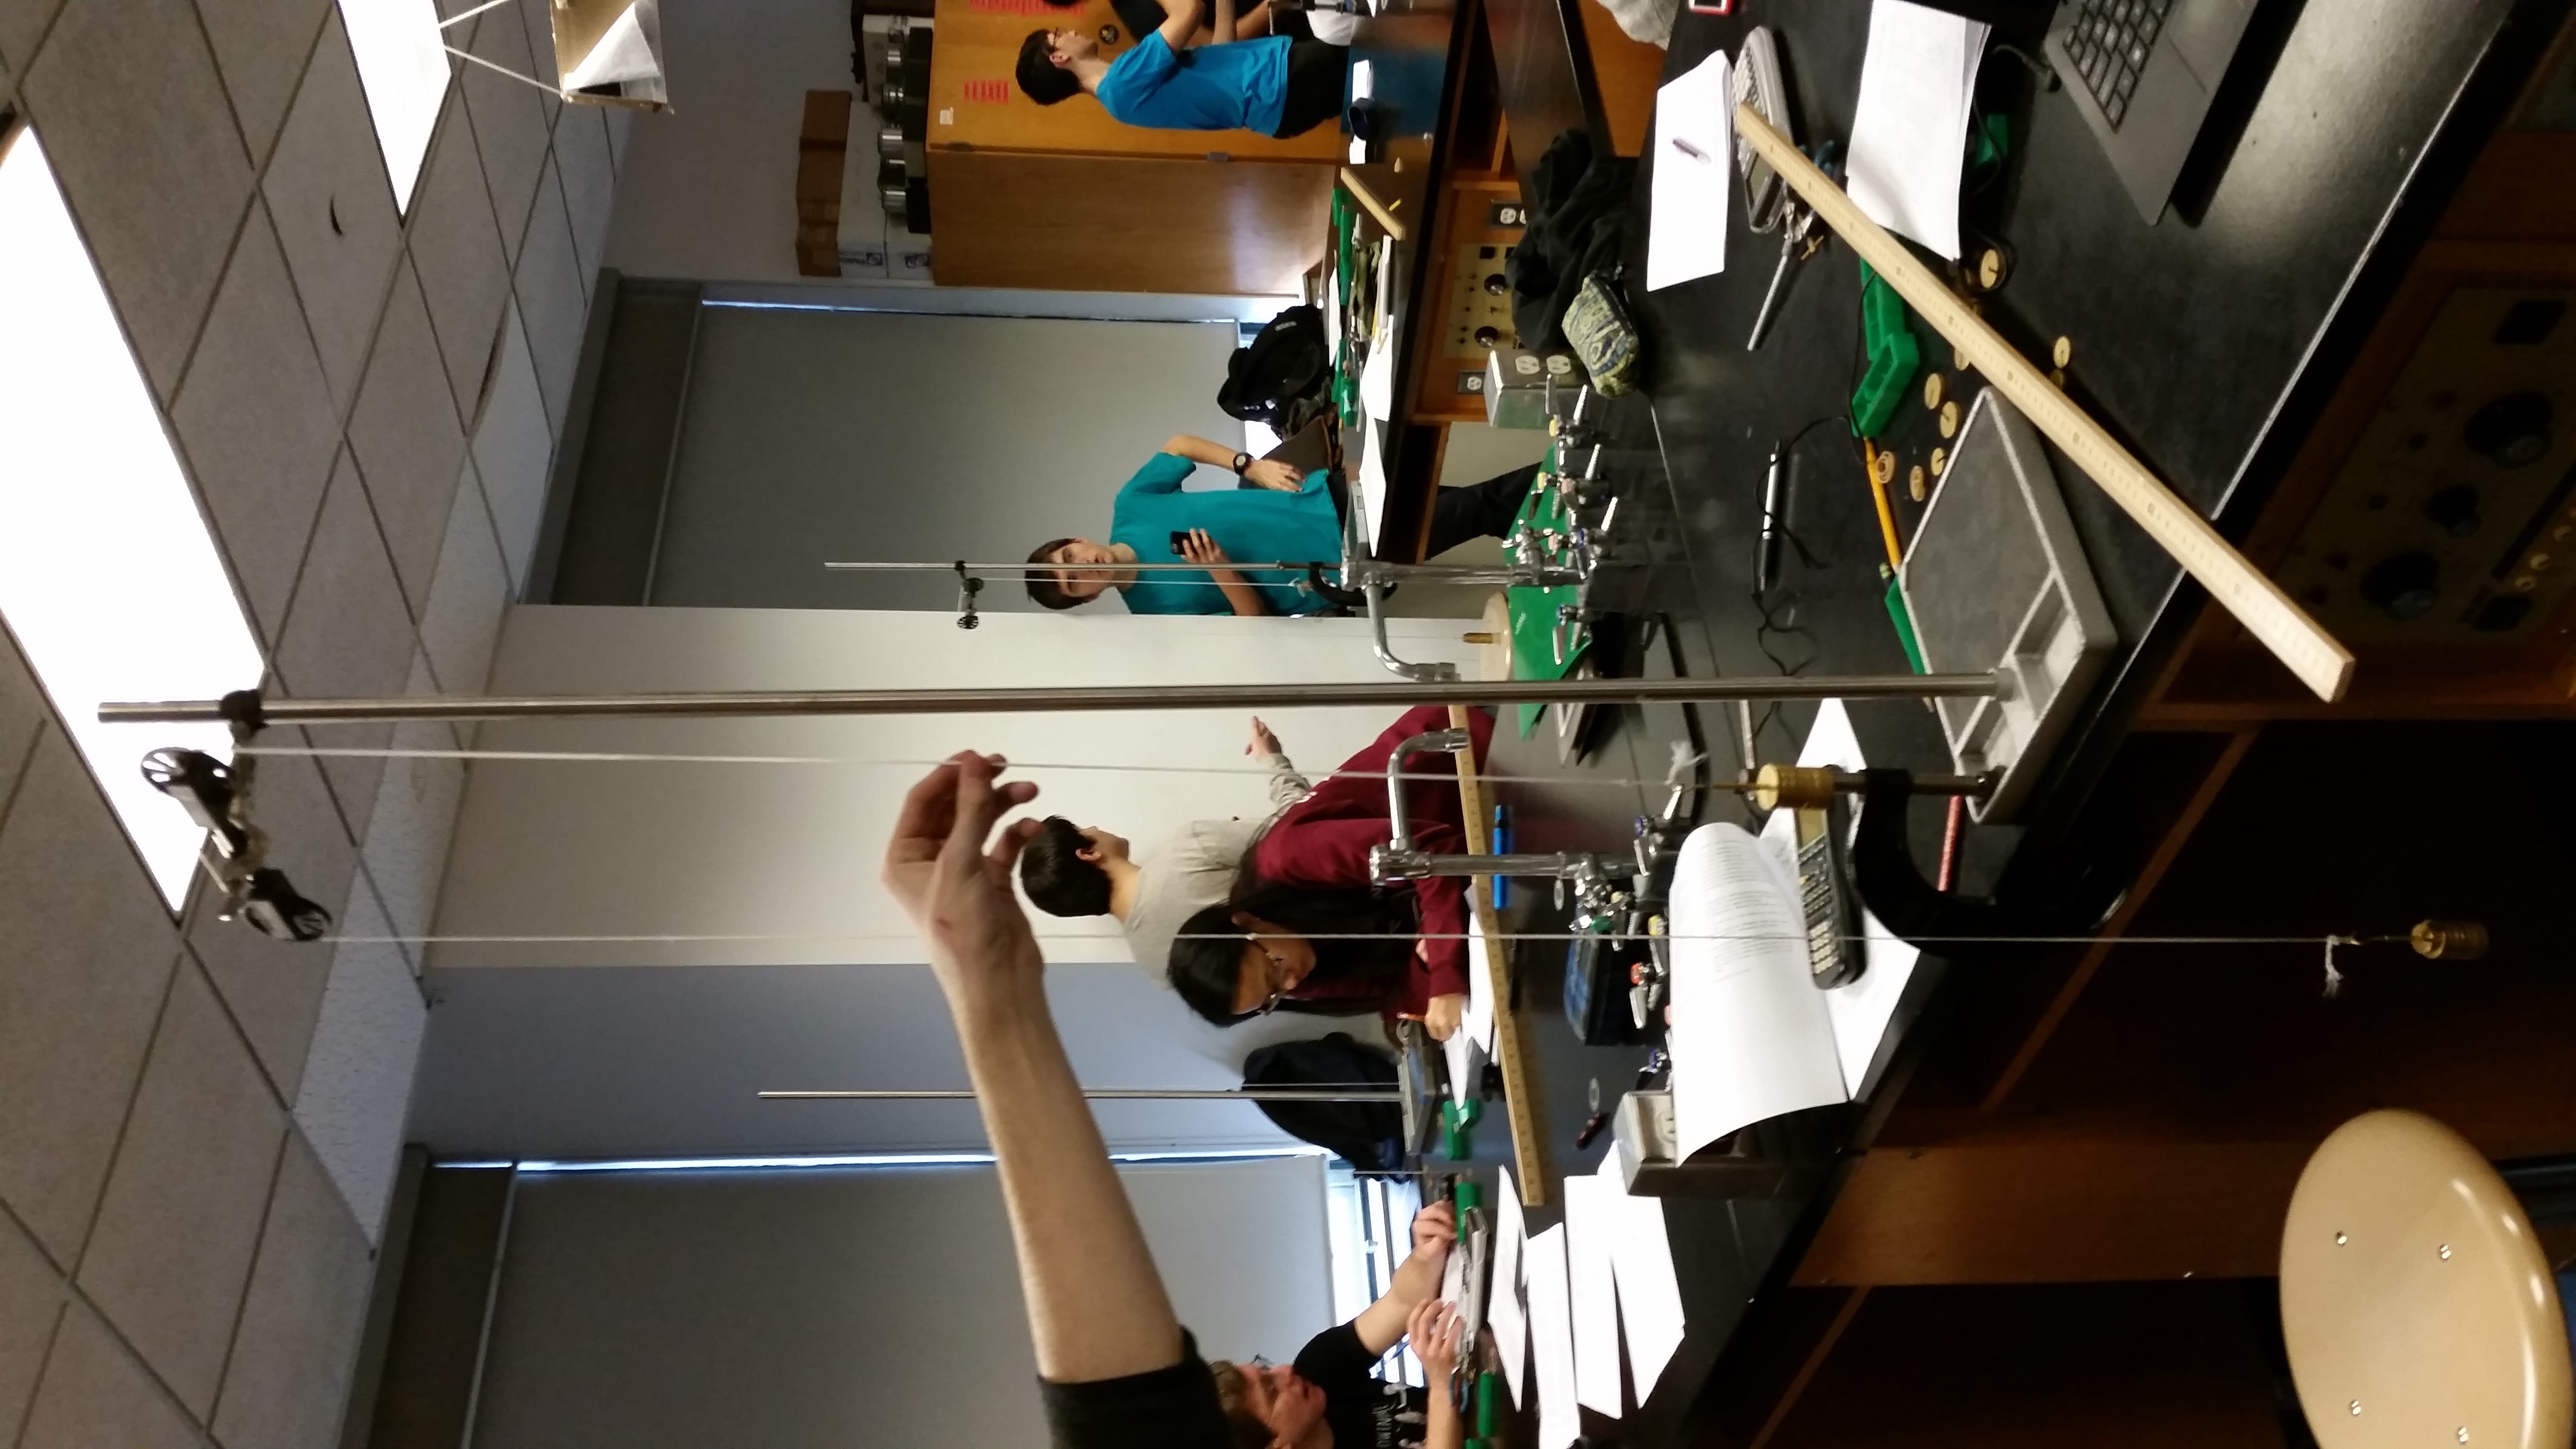
\includegraphics[scale=0.15, angle=270]{lab1.jpg}
\vspace*{1cm}
\end{figure}

\begin{center}
$$m_{pulley} = 31.6 g$$
\begin{tabular}
{|m{7em}|m{7em}|m{7em}|m{7em}|m{7em}|}
\hline
Trial & 1 & 2 & 3 & 4 \\
\hline
Descending Mass, $m_2$ (kg) & 0.06636 & 0.165 & 0.26636 & 0.3673\\
\hline
Ascending Mass, $m_1$ (kg) & 0.055 & 0.150 & 0.250 & 0.350\\
\hline
Distance of Travel, $y$ (m) & 0.8984 & 0.855 & 0.605 & 0.61\\
\hline
Time of Travel, Run 1, $t_1$ (s) & 1.47 & 2.1 & 2.54 & 3.28\\
\hline
Time of Travel, Run 2, $t_2$ (s) & 1.21 & 2.27 & 2.48 & 3.4\\
\hline
Time of Travel, Run 3, $t_3$ (s) & 1.31 & 2.18 & 2.44 & 3.55\\
\hline
Frictional Mass, $m_f$ (kg) & 0.00136 & 0.005 & 0.00636 & 0.0073\\
\hline
\end{tabular}
\begin{tabular}
{|m{7em}|m{7em}|m{7em}|m{7em}|m{7em}|}
\hline
Trial & 5 & 6 & 7 & 8 \\
\hline
Descending Mass, $m_2$ (kg) & 0.2673 & 0.2693 & 0.2713& 0.2763\\
\hline
Ascending Mass, $m_1$ (kg) & 0.259 & 0.257 & 0.255 & 0.25\\
\hline
Distance of Travel, $y$ (m) & 0.61 & 0.61 & 0.61 & 0.61\\
\hline
Time of Travel, Run 1, $t_1$ (s) & 9.16& 4.58& 2.75& 2.1\\
\hline
Time of Travel, Run 2, $t_2$ (s) & 6.35& 3.6 & 3.16 & 2\\
\hline
Time of Travel, Run 3, $t_3$ (s) & 8.15& 4.21 & 3.03 & 2.13\\
\hline
Frictional Mass, $m_f$ (kg) & 0.0073 & 0.0073 & 0.0073 & 0.0073\\
\hline
\end{tabular}
\end{center}

\section*{Discussion}
Sample calculations for the non-measured data are as shown using the formulas found above:
$$t_{avg} = \frac{t_1 + t_2 + t_3}{3} = \frac{1.47 + 1.21 + 1.31}{3} = 1.33$$
$$a = \frac{2y}{t^2} = \frac{2*0.8984}{1.33^2} = 1.015$$
$$m_t = m_1 + m_2 + m_{pulley} = 0.06636 + 0.055 + 0.0316 = 0.1529$$
$$F_{net} = (m_2 - m_1 - m_f)g = (0.06636 - 0.055 - 0.00136)(9.8) = 0.098$$
$$a_t = \frac{F_{net}}{m_t} = \frac{0.098}{0.1529} = 0.64$$
$$\text{Percent Acceleration Error} = \frac{|a_t - a_m|}{a_t}*100\% = \frac{|0.64 - 1.015|}{0.64}*100\% = \frac{0.375}{0.64}*100\% = 58.59\%$$

\begin{center}
\begin{tabular}
{|m{7em}|m{7em}|m{7em}|m{7em}|m{7em}|}
\hline
Trial & 1 & 2 & 3 & 4 \\
\hline
Average Time, $t_{avg}$ (s) & 1.33 & 2.183 & 2.486 & 3.41\\
\hline
Measured Acceleration, $a_m$ ($kgm/s^2$) & 1.015 & 0.359 & 0.196 & 0.105\\
\hline
Total Mass, $m_t$ (kg) & 0.1529 & 0.3466 & 0.547 & 0.7489\\
\hline
Net Force, $F_{net}$ (N) & 0.098 & 0.163 & 0.149 & 0.098\\ 
\hline
Theoretical Acceleration, $a_t$ ($kg*m/s^2$) & 0.64 & 0.47 & 0.27 & 0.131\\
\hline
Percent Acceleration Error (\%) & 58.59 & 23.62 & 27.4 & 19.7\\
\hline
\end{tabular}
\begin{tabular}
{|m{7em}|m{7em}|m{7em}|m{7em}|m{7em}|}
\hline
Trial & 5 & 6 & 7 & 8 \\
\hline
Average Time, $t_{avg}$ (s) & 7.88 & 4.13 & 2.98 & 2.076 \\
\hline
Measured Acceleration, $a_m$ ($m/s^2$) & 0.0196 & 0.0715 & 0.137& 0.283\\
\hline
Total Mass, $m_t$ (kg) & 0.5589 & 0.5589 & 0.5589 & 0.5589\\
\hline
Net Force, $F_{net}$ (N) & 0.0098 & 0.049 & 0.0882 & 0.1862\\ 
\hline
Theoretical Acceleration, $a_t$ ($m/s^2$) & 0.0175 & 0.0877 & 0.158 & 0.333 \\
\hline
Percent Acceleration Error (\%) & 12 & 18.5 & 13.3 & 15.01 \\
\hline
\end{tabular}
\end{center}

Our percent error was fairly high for the first set of data, especially as the mass was lower, most likely indicating an issue with the time measurement, as it was faster at the start, at which points the percent of error was far higher. 

Other sources of error that could have occured was within the pulley mechanism itself, estimating the frictional mass manually, which created room for error, and it assumes that the pulley itself worked as intended, although there was the chance of it slipping or catching at any point. In addition, there is the possibility of drag force slowing the measured acceleratin, which is consistent with the data, except in the 1st and 5th trial.

Finally, the equations themselves assumed a point mass, while in actuality, as the masses got higher, they became less and less point-like in shape, interfering in the data.

\section*{Conclusion}

The acceleration as the mass on each side before frictional mass was added increased from 0.05 to 0.15 to 0.25 to 0.35, went from 1.015 $m/s^2$ with 58.59\% error, to 0.359 $m/s^2$ with 23.62 \% error, to 0.196 $m/s^2$ with 27.4 \% error, to 0.105 $m/s^2$ with 19.7\% error.

The acceleration as the mass difference increased from 2 g to 6 g to 10 g to 20 g, went from 0.0196 $m/s^2$ with 12 \% error, to 0.0715 $m/s^2$ with 18.5 \% error, to 0.137 $m/s^2$ with 13.3 \% error, to 0.283 $m/s^2$ with 15.01 \% error. 

\end{document}
